\chapter{Ejercicio 2 }
\part{Ejercicio 2}
\section{Enunciado}
La empresa Musimundo cuenta con una serie de sucursales repartidas por el pa'is. Recientemente ha decidido cerrar su sucursal
de Iruya y llevarse toda la mercader'ia al dep'osito central. Debido al dif'icil acceso ha dispuesto s'olo un cami'on para
llevar toda la mercader'ia. Sin embargo, es posible que no todo el material pueda ser llevado en un s'olo viaje del cami'on
d'ebido a las restricciones de carga, por lo que la parte que no entre en el cami'on ser'a vendida a valores despreciables el
 d'ia del cierre.
Dada la capacidad de carga m'axima P del cami'on y una lista de los productos del local conteniendo el valor $v_i$ y peso $p_i$ 
de cada uno, encontrar la lista de productos de mayor valor que sea posible llevar en el cami'on sin que el peso total de la
lista supere la carga m'axima. El valor de una lista de productos se calcula como la suma de los valores de los productos
involucrados. En caso de haber varias listas con el mismo valor m'aximo, encuentre cualquiera de ellas.
Realice un algoritmo para resolver el problema usando la t'ecnica de backtraking.

\section{Desarrollo}
Dado que el problema deb'ia ser resuelto con backtracking, buscamos la forma de aplicar dicha t'ecnica algor'itmica para su resoluci'on. B'asicamente la idea es formar todos los subconjuntos de cosas para encontrar aquel que maximice el valor total.\\ 
La restricci'on explicita es el conjunto de cosas a llevar y la restricci'on implicita es la capacidad de carga del cami'on. A 
medida que se va armando una soluci'on, son descartadas aquellas cuya suma es mayor al peso que puede transportar el cami'on, de 
esta manera se va podando el 'arbol de posibles soluciones.
De esta manera, se construye el siguiente 'arbol de recursion:
\begin{figure}[H]
\centering
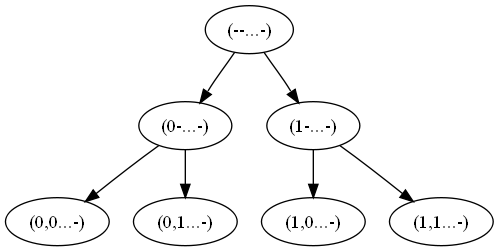
\includegraphics[scale=0.5]{./ejercicio2/arbol.png}
\end{figure}
En la raiz del 'arbol se tiene la solucion conjunto vacio. Luego en cada nodo se tiene una $n-upla$ donde un $0$ en la posicion $i$ 
indica que el elemento $i$ no se lleva, y un $1$ indica que el elemento se lleva. Las hojas de este 'arbol son las soluciones 
posibles. Como cada elemento puede estar o no estar, se tienen dos posibilidades para cada uno (llevarlo o no), esto implica que la cantidad 
posible de soluciones si se tienen $n$ elementos es $2^n$.\\
El algoritmo implementado toma como parametros las cosas que se pueden llevar, dos soluciones posibles, una en donde esta guardada la mejor 
encontrada hasta el momento y otra que guarda la que se va construyendo, asi tambien el peso maximo que se puede llevar y un indice que 
indica sobre que cosa se esta decidiendo llevar o no.\\
Basicamente una llamada a la funci'on consiste en verificar si se agrega o no a la solucion el elemento apuntado por indice, si es asi, es 
decir que al agregarlo, el peso total no exede el peso maximo, se agrega a la soluci'on candidata, luego de esto se continua con la siguiente llamada recursiva. Esta consiste en una llamada sin agregar el elemento apuntado por indice. Cuando se encuentra una soluci'on mejor a la optima actualmente, esta es reemplazada. Repitiendo este proceso se pueden observar todas las hojas del arbol, para quedarse con la mejor.\\  

Para implementar el algoritmo se definieron los tipos: Cosa, Camion y SolucionPosible. Con la finalidad de aportar mas claridad al mismo.

\section{Pseudocodigo}
\noindent
SolucionPosible: tupla$<cantCosas, guardo:[bool], valor, costo>$ \\
Camion: tupla$<cantCosas, capacidad, cosas: [Cosa]>$ \\
Cosa: tupla$<costo, valor>$ \\
cosas = $\{a_1,....,a_{cant}\}$ \\

\begin{algorithm}
\caption{Halla la soluci'on 'optima al problema del camion}
\begin{algorithmic}[1]
    \STATE s $\textcolor{orange}{\leftarrow}$ SolucionPosible\textcolor{magenta}{(}cant cosas\textcolor{magenta}{)}
    \STATE ordenar arreglo de cosas \COMMENT{mediante merge sort}
    \STATE valorMaximo $\textcolor{orange}{\leftarrow}$ $\sum_{t=0}^{cant cosas} \textcolor{magenta}{(}cosa_i\textcolor{magenta}{)}_{valor}$ 
    \STATE camionAux\textcolor{magenta}{(}s,c,0,mejorSol,valorMaximo\textcolor{magenta}{)}
\end{algorithmic}
\end{algorithm}

\begin{algorithm}
\caption{camionAux: Halla la solución óptima $mejorSol$ al problema del camion}
\begin{algorithmic}[1]
    \IF{ prob'e con las cant cosas \textcolor{orange}{\&} valor\textcolor{magenta}{(}candActual\textcolor{magenta}{)} $\textcolor{orange}{>}$ valor\textcolor{magenta}{(}mejorSol\textcolor{magenta}{)} }
        \STATE mejorSol $\textcolor{orange}{\leftarrow}$ candActual
        \STATE terminar
    \ENDIF    
    \IF{el valor del actual $\textcolor{orange}{+}$ valorMaximo $\textcolor{orange}{\leq}$ el valor de la mejor soluci'on hasta el momento}
        \STATE terminar
    \ELSE
        \IF {no prob'e las cant cosas}
                \IF {no me paso del peso máximo agregando $a_i$ a candActual}
                    \STATE agregar\textcolor{magenta}{(}$a_i$, candActual\textcolor{magenta}{)}
                    \STATE camionAux\textcolor{magenta}{(}candActual, cosas, capacidad, i\textcolor{orange}{+}1, cant, mejorSol\textcolor{magenta}{)}
                    \STATE sacar\textcolor{magenta}{(}$a_i$, candActual\textcolor{magenta}{)}
            		\ELSE
            								\STATE \COMMENT{ como los demas pesan mas, no puedo agregar a mas nadie}
		   	        						\IF{ valor\textcolor{magenta}{(}candActual\textcolor{magenta}{)} $\textcolor{orange}{>}$ valor\textcolor{magenta}{(}mejorSol\textcolor{magenta}{)} }
       											  	\STATE mejorSol $\textcolor{orange}{\leftarrow}$ candActual
        										\ENDIF	       
        										\STATE terminar
        				\ENDIF
         \STATE camionAux\textcolor{magenta}{(}candActual, cosas, capacidad, i\textcolor{orange}{+}1, cant, mejorSol\textcolor{magenta}{)}
    \ENDIF
   \ENDIF
\end{algorithmic}
\end{algorithm}

%TODO: completar esta demostracion, hablar de tama�o de entrada. Tarea de fede
%hablar de peor caso
\section{C'alculo de complejidad}
Para este ejercicio decidimos usar el modelo uniforme, ya que consideramos que lo que hace al n'ucleo del problema es la
cantidad de cosas a llevar. Por esa razon no nos parece desacertado considerar que el peso y el valor de las cosas estan 
acotados. Asi mismo consideraremos que el tama\~{n}o de la entrada es la cantidad de cosas que se pueden llevar.\\
Para nuestro algoritmo, el peor caso se da cuando no puedo podar ninguna rama, es decir cuando se deben llevar todos los elementos, ya que entonces lo que hacemos es revisar las $2^n$ posibles soluciones.
Observando el pseudocodigo podemos notar que la ecuacion de recurrencia es la siguiente:\\
%TODO: hacer la demo
$T(0) = 1$\\
$$T(n) = 2*T(n-1) + k$$\\
Ya que hacemos dos llamadas con el indice incrementado en una posicion.\\
El algoritmo resulta tener una complejidad asintotica en peor caso de $O(2^n)$. La demostraci'on de dicha afirmacion, es la siguiente:\\
Queremos probar que $T(n) \in O(2^n)$. Para esto planteamos las siguientes igualdades:\\
$$a: T(n) = 2*T(n-1) + k$$\\
$$b: T(n+1) = 2*T(n) + k$$\\
Luego restamos $a$ con $b$ y dejamos todo de un lado de la igualdad y nos queda:\\
$$T(n+1) - 3*T(n) + 2*T(n-1) = 0$$\\
Con esto usamos las ecuaciones caracter'isticas, dando resultado al siguiente polinomio:\\
$$x^2 - 3*x + 2 = 0$$\\
Cuyas raices son $x = 1$ y $x = 2$. Con estos datos, $T(n)$ tiene la siguiente forma:\\

\centerline{$T(n) = A*1^n + B*2^n = A + B*2^n$  para A y B constantes}

\medskip
Luego queda claro que $T(n) \in O(2^n)$.

Para nuestro algoritmo el peor caso es cuando hay que llevar todos los elementos, ya que no se puede hacer poda en ningun momento. En este caso probara con todas las combinaciones hasta que quede que la mejor solucion era llevar todo. Ocurre lo contrario si no hay que llevar ningun elemento, ya que en cada paso hace solo una llamada recursiva(es decir la que no incluye al elemento actual)
%TODO: hablar de cual es el peor caso

\section{Analisis Experimental}
\subsection{Experiencias realizadas}
Para probar el comportamiento del algoritmo, se procedi'o a medir los tiempos y la cantidad de operaciones. En ambos casos se generaron muestras con un numero creciente de elementos (las caracteristicas de la muestra fueron generadas al azar) y por otro lado se hizo un analisis del peor caso. Como se dijo anteriormente, el peor caso se da cuando no se puede podar ningun elemento, por lo tanto, es necesario ver todas las soluciones(es decir, recorrer todo el arbol).
Cuando fue posible, se utiliz'o la tecnica de cuadrados minimos para buscar una funci'on que aproxime a las observaciones obtenidas, para graficar dicha funci'on y contrastarla con las observaciones.

\subsection{Gr'aficos}
%TODO: sergio hace los graficos con n creciente y aleatorio

\begin{figure}[H]
\centering
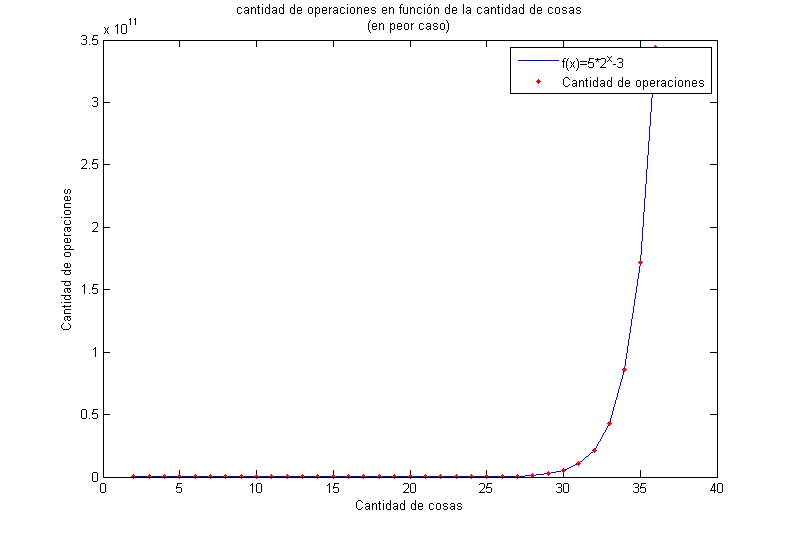
\includegraphics[scale=0.8]{../../codigo/ejercicio2/benchmark/graficos/operaciones_peor_caso/cantOperacionesPeorCaso.png}
\caption{Cantidad de operaciones en funcion de la cantidad de cosas en peor caso}
\end{figure}

\begin{figure}[H]
\centering
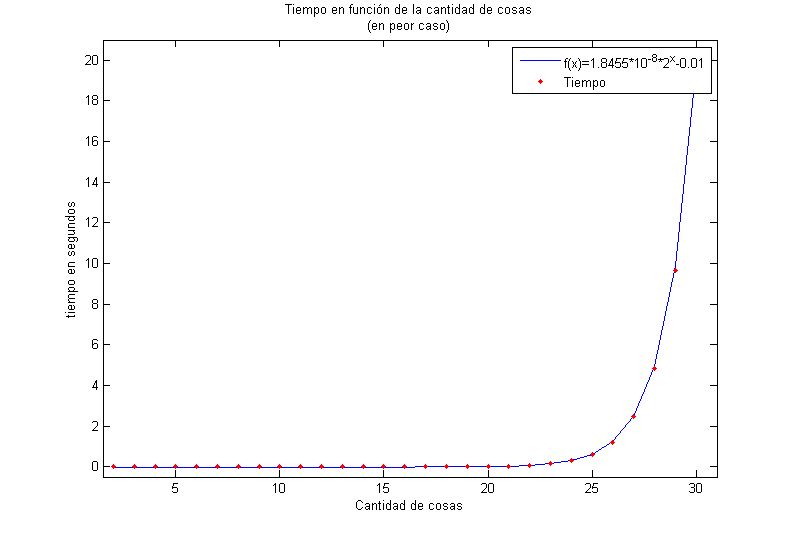
\includegraphics[scale=0.8]{../../codigo/ejercicio2/benchmark_tiempos/graficos/tiempo_peor_caso/tiempobackTracking.png}
\caption{Tiempo en funcion de la cantidad de cosas en peor caso}
\end{figure}

\begin{figure}[H]
\centering
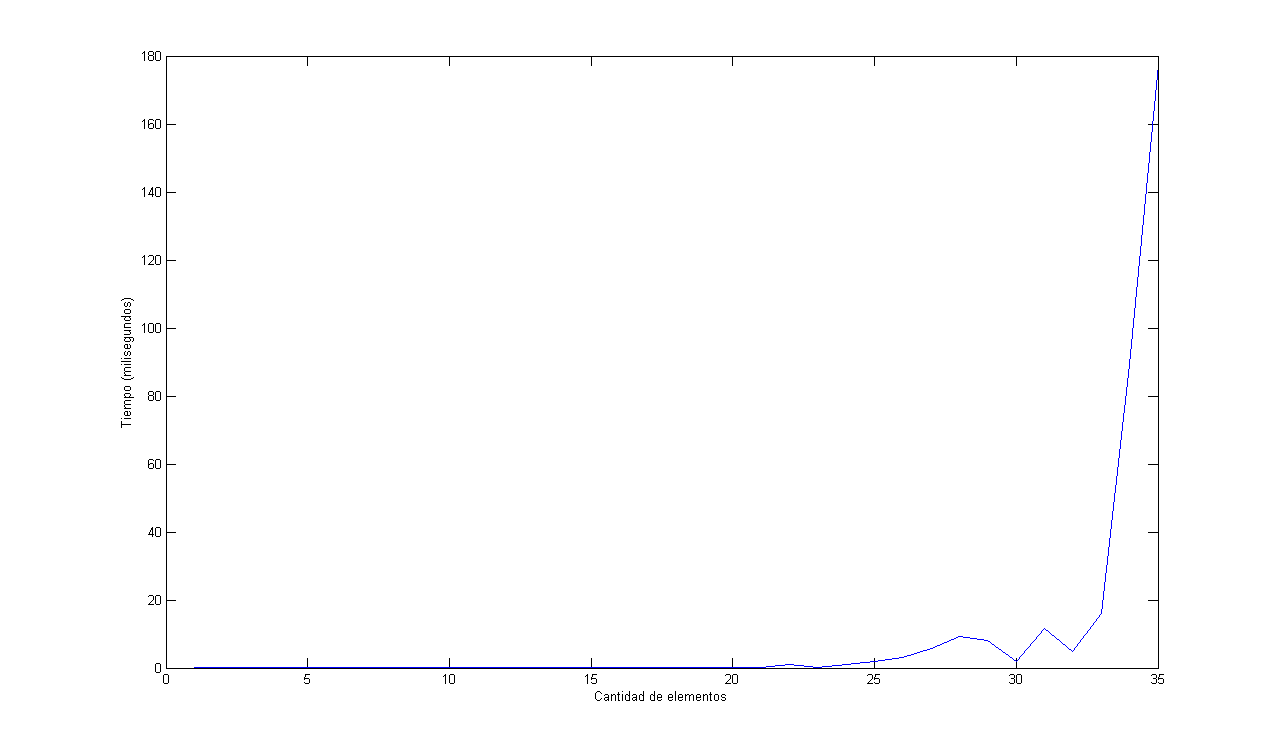
\includegraphics[scale=0.8]{../../codigo/ejercicio2/benchmark_tiempos/graficos/tiempo_aumentando_cant_articulos/aumentandoCantArticulosPromedio.png}
\caption{Tiempo en funcion de la cantidad de cosas (peso y valor aleatorios con distribucion uniforme)}
\end{figure}

\section{Discusi'on}


	
